\providecommand{\main}{..}
\documentclass[../mthe-493-final-project.tex]{subfiles}

%Full analysis of results, against optimization constraints, and model measures like accuracy, staleness etc.

\begin{document}
    \chapter{Results \& Analysis}
    \label{ch:results-and-analysis}
    
    \section{Benchmarking}
    \label{sec:benchmarking-results}
    %This may be best first, since it lets the reader now what accuracy the parameters fed into the optimization held.
    
    To assess the performance of benchmarking results, sets of experiments were devised wherein some system parameters were varied, and others were held constant. After repeating the experiments numerous times, some key metrics regarding benchmarking accuracy were deduced.
    
    In the following figure, the ratio of actual computation time (incl. orchestrator overhead) and network time to maximum training time $T$ is shown, stratified by the values of $T$. These values were taken over 200 experiments using anywhere between 1 and 8 learners.
    
    \begin{figure}
        \centering
        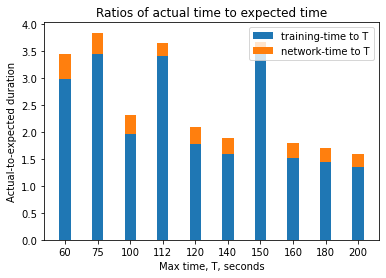
\includegraphics[width=120mm,scale=0.5]{thesis/img/benchmarking-error-by-max-time.png}
        \caption{Ratio of network and training time to maximum time}
        \label{fig:benchmarking-results-1}
    \end{figure}
    
    \autoref{fig:benchmarking-results-1} suggests that, generally, the network time is contributes a static overhead to overall experiment run time. However, it is still significant in that it may require 20\% - 40\% of the overall run time. This is a large factor that is not accounted for in benchmark models.
    
    The actual training time, including orchestrator overhead, tends to be 50\% - 250\% \textit{more} than the maximum training time. 
    
    Now, only the actual learner times (training time less orchestrator overhead) are taken as a ratio to max training time $T$, stratified again by $T$. For each experiment, the average learner compute time and the maximum (slowest) learner compute times are considered across all global updates in said experiment. Again, these experiments were repeated multiple times for each $T$, thus the average of the ratios for each scenario across multiple experiments are shown.
    
    \begin{figure}
        \centering
        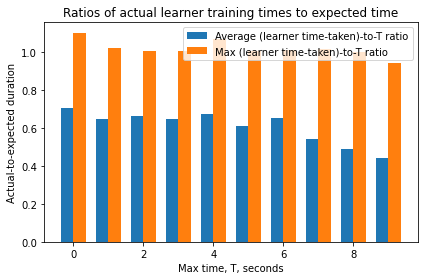
\includegraphics[width=150mm,scale=0.5]{thesis/img/average-max-learner-actual-times.png}
        \caption{Ratio of average and slowest worker actual times to maximum time}
        \label{fig:benchmarking-results-2}
    \end{figure}
    
    \autoref{fig:benchmarking-results-2} displays some results that are crucial to understanding the accuracy of the benchmarking system. We see from the data set of average-case performance, the benchmarking is generally accurate. However, the system is fundamentally slowed down by the slowest worker, if they are assigned more data than can be computed within their allotted time. These situations can be seen where the max ratio exceeds 1.0.
    
    When both figures are taken together, it is clear that the learner estimations are sufficiently accurate (\autoref{fig:benchmarking-results-2}, but there is a significant oversight in the modelling of the expected vs. actual total system time, as per \autoref{fig:benchmarking-results-1}. Thus, more effort needs to be put towards modelling the orchestrator and network overhead.
    
    \section{Optimization}
    
    The development of both Gurobi and heuristic implementations as decided in \autoref{sec:optimization-engineering-tools} requires an assessment of
    \begin{itemize}
        \item validity and optimality of solutions generated, and
        \item run-time analysis
    \end{itemize}
    between both optimizers.
    
    The testing infrastructure developed in \autoref{ssection:optimization-optimizer-implementation-evaluation} was employed to run both optimizers under an identical test set of 10,000 randomly generated experiments.
    
    \subsection{Validity \& Optimality of Solutions}
    
    To test the efficacy of the heuristic optimization model, the solutions it produced in 10,000 experiments with varying parameters were compared against the solutions achieved by the Gurobi optimization tool. In 9.64\% of experiments both systems returned that there were no feasible points to the integer programming problem. Further, in all 10,000 experiments there were no disagreements between the models regarding problem feasibility. This indicates that the feasibility checks built into the heuristic model are completely exhaustive.
    
    
    \begin{figure}
        \centering
        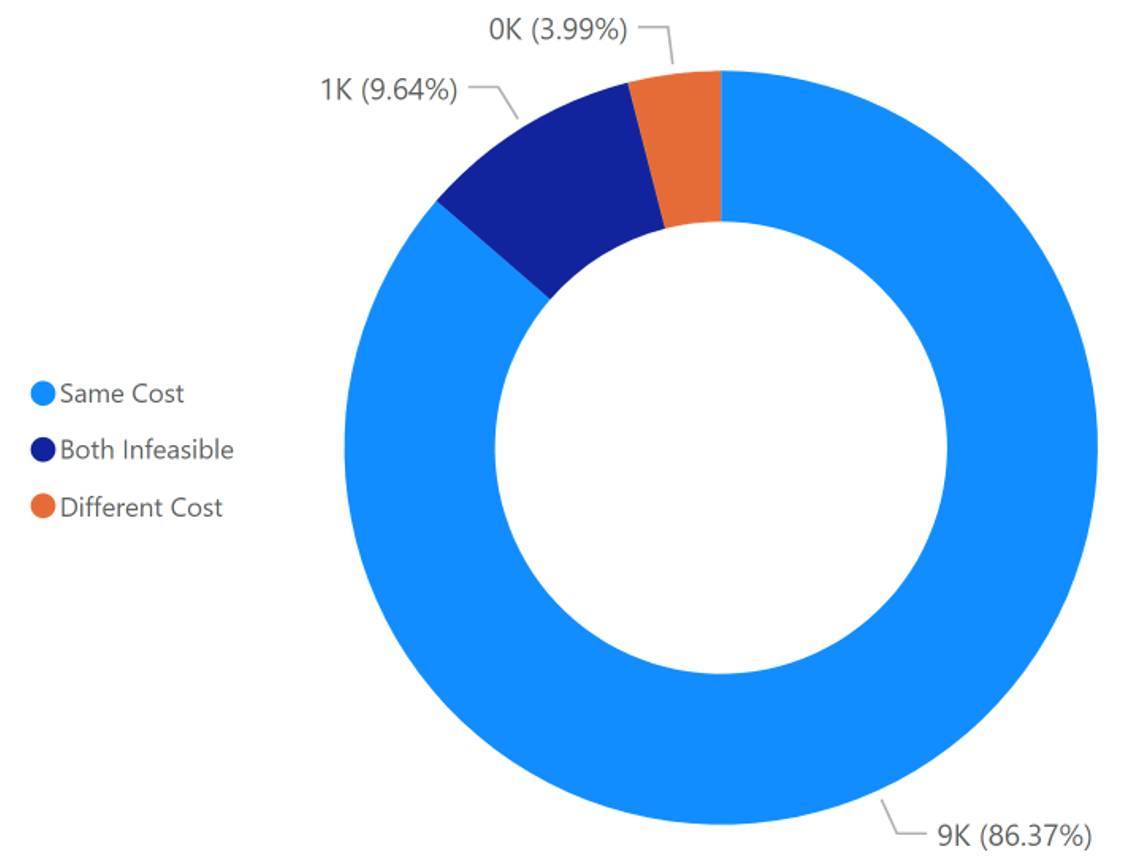
\includegraphics[width=120mm,scale=0.5]{optimization-results-1.png}
        \caption{Heuristic and Gurobi cost comparison over 10K experiments.}
        \label{fig:optimization-results-1}
    \end{figure}
    
    In 86.37\% of the 10,000 experiments both frameworks came to the same solution for minimal total deployment cost. This means that in 95.59\% of the cases where there was a feasible solution, both processes achieved the same optimum.
    
    In 4.42\% of the experiments for which there was a feasible solution, Gurobi and the heuristic model produced different results. Of these experiments, Gurobi achieved a lesser value in 49\%, while the heuristic model outperformed in the other 51\%.
    
    \begin{figure}
        \centering
        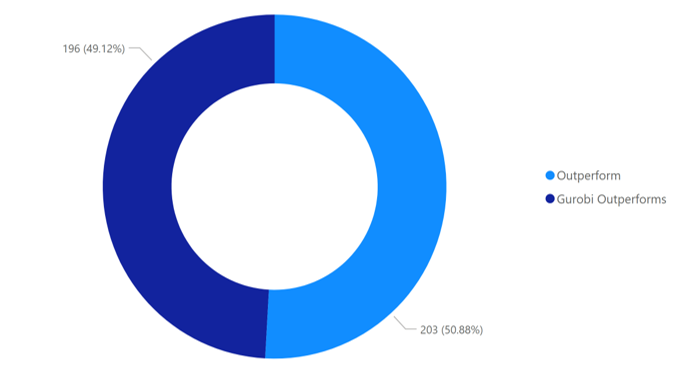
\includegraphics[width=150mm,scale=0.5]{optimization-results-2.png}
        \caption{Heuristic and Gurobi lower cost comparison in experiments with different results.}
        \label{fig:optimization-results-2}
    \end{figure}

    The fraction of cases where Gurobi outperforms is likely due to a small edge case which is not captured by the heuristic process. Conversely, in the cases where the heuristic model achieves a lower minimum for the objective function, it is speculated that this may be due to minute sacrifices in the accuracy of Gurobi's general-purpose optimizer in turn for speed increases. This cannot be confirmed because the Gurobi software is completely closed-source.
    
    Ultimately, the average difference between total costs in the experiments where the models produced different solutions was only 0.1\%. The largest recorded difference in total cost in a single experiment was 4\%.
    
    Since Gurobi is a widely trusted and reputable optimization engine~\cite{gurobi}, these results indicate that the heuristic model is also highly proficient as an optimizer.
    
    \subsection{Run-time Analysis}
    
    The run-time analysis was a simple assessment to make; the total run-time was recorded for each optimizer whilst executing the set of experiments. It was found that Gurobi's implementation ran for an average of 11.58 seconds per test case. The heuristic algorithm achieved a remarkable average of 3.9 seconds per test case, a nearly three-fold reduction in run-time on identical data sets.
    
    When taken alongside the comparable rate of suboptimal solutions, qualitative merits discussed in \autoref{sssec:optimization-candidate-heuristic}, and the superior run-time, the heuristic algorithm was correctly selected as the best candidate for the implementation of an optimization solver in the project.
    
    \section{Parallel Learning}
    Due to some last-minute issues with the proposed network of Raspberry Pis, we were unable to run our solution on those devices. Unfortunately, the is were just not capable of performing the computations necessary to train a neural network. This is despite selecting the incredibly lightweight MNIST 2NN network architecture. As a result, the Pis were swapped out for the personal computers of our group \& friends. This created an issue as the learners must all be connected to the same network in order to run our solution. For this reason, the following results and analysis have been segmented into two sections: the presentation set and the thesis set. Presentation testing was limited to a set of maximum 5 learners whereas thesis testing made use of 8 learners.

    Prior to jumping into results, it’d be helpful to define two variables that will be referenced throughout. The minimum number of learners that will receive a fraction of the dataset will be known as beta. The minimal number of 32 image batches that a learner receives will be known as $s_{min}$.
    
    The first area of experimentation was training to convergence. Unlike single device training, parallel learning introduces the added challenge of model aggregation which can reduce the ceiling on model accuracy, but more relevantly tends to delay convergence. The first test from the presentation set represented in figures \ref{fig:res_1} \& \ref{fig:res_2} shows the average test accuracy and loss from 50 training cycles taken to 100 global updates. This test was completed at the presentation set maximum of beta equal to five \& $s_{min}$ equal to 128. Model accuracy reached 97\% after 80 global updates and only managed to improve .1\% to 97.1\% after the 100\textsuperscript{th} global update. Further, beyond 80 updates our loss and accuracy plots were no longer strictly decreasing and increasing respectively. Oscillation of both metrics and nearly 0 slope were observed past the 80-update threshold making it an excellent estimate for convergence.
    \begin{figure}
        \centering
        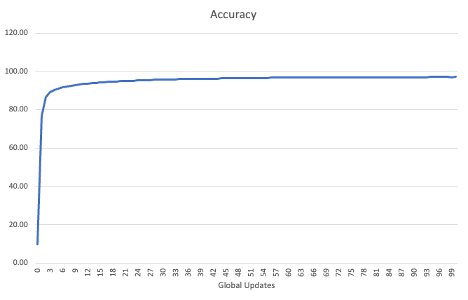
\includegraphics[width=150mm]{thesis/img/res_1.png}
        \caption{Average accuracy over 50 tests to 100 global updates.}
        \label{fig:res_1}
    \end{figure}
    \begin{figure}
        \centering
        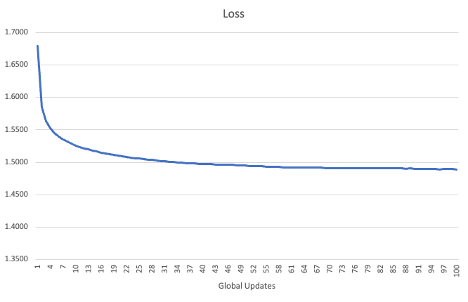
\includegraphics[width=150mm]{thesis/img/res_2.png}
        \caption{Average loss over 50 tests to 100 global updates.}
        \label{fig:res_2}
    \end{figure}
    These results were replicated in figures \ref{fig:res_3} \& \ref{fig:res_4} where beta was now fixed at the thesis set maximum of 8. From this we can conclude that within the scope of our project, 80 global cycles are an excellent estimate for convergence.
    \begin{figure}
        \centering
        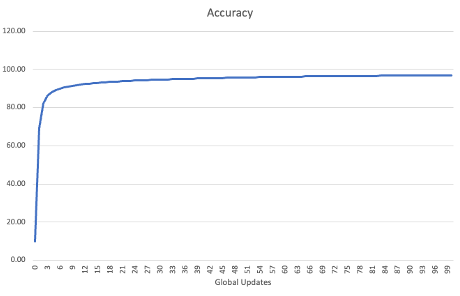
\includegraphics[width=140mm]{thesis/img/res_3.png}
        \caption{Average accuracy over 50 tests to 100 global updates.}
        \label{fig:res_3}
    \end{figure}
    \begin{figure}
        \centering
        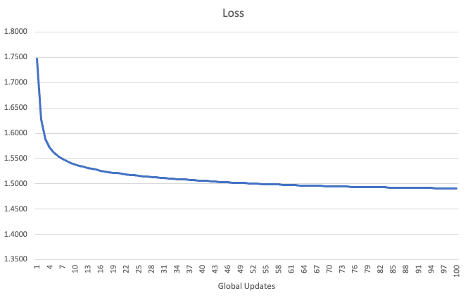
\includegraphics[width=140mm]{thesis/img/res_4.png}
        \caption{Average loss over 50 tests to 100 global updates.}
        \label{fig:res_4}
    \end{figure}
    The next area of experimentation was a varied beta value for a fixed $s_{min}$ of 128. We looked for its impact on both metrics of loss and accuracy as the number of learners increased. Going in, the group hypothesized that it would be more challenging to aggregate the parameters of more models. Further, this kind of behaviour was partially exhibited in our weight initialization experimentation. However, our hypothesis was proven to be entirely incorrect in our presentation set. As seen in figures \ref{fig:res_5} \& \ref{fig:res_6} where loss and accuracy have been plotted to our estimated convergence of 80 global updates, there is no notable drop in accuracy or jump in loss as beta increases from two to five. 
    \begin{figure}
        \centering
        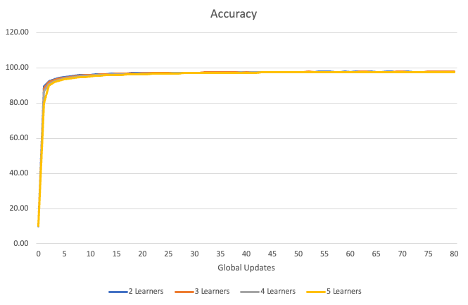
\includegraphics[width=120mm]{thesis/img/res_5.png}
        \caption{Accuracy to estimated convergence for varied beta.}
        \label{fig:res_5}
    \end{figure}
    \begin{figure}
        \centering
        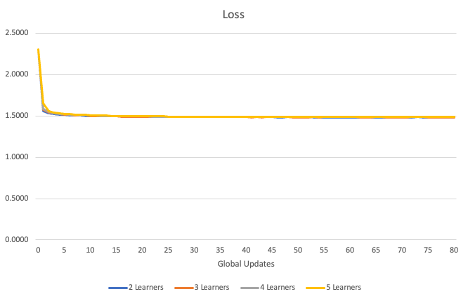
\includegraphics[width=120mm]{thesis/img/res_6.png}
        \caption{Loss to estimated convergence for varied beta.}
        \label{fig:res_6}
    \end{figure}
    Further, the final test accuracies at estimated convergence are within .5\% of each other and the final values of loss are within 4 thousandths of each other as seen in figures \ref{fig:res_7} \& \ref{fig:res_8}. 
    \begin{figure}
        \centering
        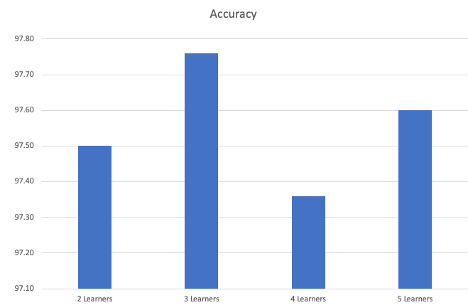
\includegraphics[width=138mm]{thesis/img/res_7.png}
        \caption{80\textsuperscript{th} global update accuracy for varied beta.}
        \label{fig:res_7}
    \end{figure}
    \begin{figure}
        \centering
        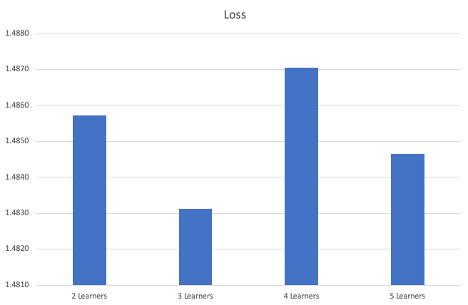
\includegraphics[width=138mm]{thesis/img/res_8.png}
        \caption{80\textsuperscript{th} global update loss for varied beta.}
        \label{fig:res_8}
    \end{figure}
    Initially it appeared the thesis set would further disprove our hypothesis as figures \ref{fig:res_9} \& \ref{fig:res_10} look exactly like figures \ref{fig:res_5} \& \ref{fig:res_6} from the presentation set. However, when we zoom in to final test accuracy and loss in figures \ref{fig:res_11} \& \ref{fig:res_12}, clear trendlines can be drawn. Excluding what appears to be an outlier in the 4-learner experiment, test accuracy falls, and loss rises as beta increases. It’s in our group’s opinion that these results would be reproduced as the maximum beta value climbs. Once again, it’s crucial to point out that final accuracies fall within <.5\% \& values of loss within 4.5 thousandths of each other. This is an indication that the intelligent weighted averaging algorithm from FedAvg was implemented successfully in our project \& fantastically serves our use case.
    \begin{figure}
        \centering
        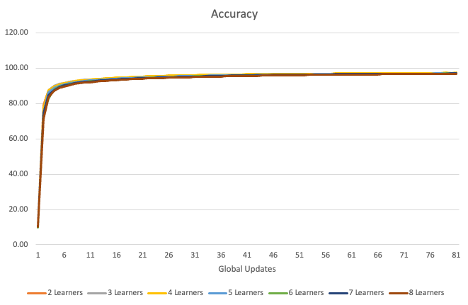
\includegraphics[width=115mm]{thesis/img/res_9.png}
        \caption{Accuracy to estimated convergence for varied beta.}
        \label{fig:res_9}
    \end{figure}
    \begin{figure}
        \centering
        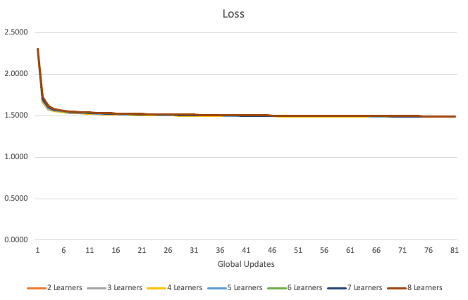
\includegraphics[width=115mm]{thesis/img/res_10.png}
        \caption{Loss to estimated convergence for varied beta.}
        \label{fig:res_10}
    \end{figure}
    \begin{figure}
        \centering
        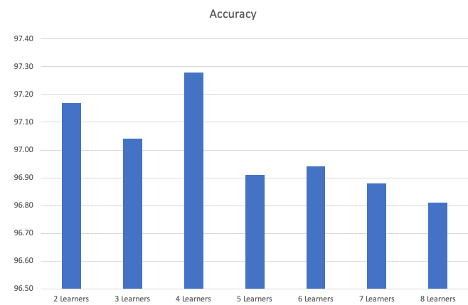
\includegraphics[width=150mm]{thesis/img/res_11.png}
        \caption{80\textsuperscript{th} global update accuracy for varied beta.}
        \label{fig:res_11}
    \end{figure}
    \begin{figure}
        \centering
        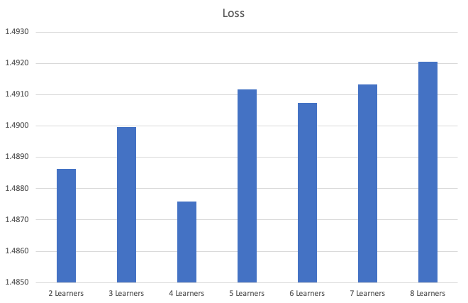
\includegraphics[width=150mm]{thesis/img/res_12.png}
        \caption{80\textsuperscript{th} global update loss for varied beta.}
        \label{fig:res_12}
    \end{figure}
    The final area of experimentation was a varied $s_{min}$ value for a fixed beta. Its impact on both test accuracy and loss were examined as before. A crucial stipulation for these experiments was that the maximum acceptable time for a learner to complete its local update was increased to ensure any given learner could receive the entire dataset less the mandatory work assigned to all other learners. This made sure that tests were performed as anticipated, and our intelligent optimization algorithm used to partition the dataset did not redistribute batches. For this experiment, the group hypothesized that as $s_{min}$ decreased and approach a single batch, we’d see an increase in test accuracy and a decrease in loss. The rationale for our hypothesis was the weighted averaging performed by the FedAvg algorithm. As some learners begin to receive inconsequentially small fractions of the dataset, their impact on the global model would go to zero. In turn, the learner with the best cost would perform nearly single device training on almost the entire dataset. Once again, we were proven wrong as can be seen in figures \ref{fig:res_13} \& \ref{fig:res_14}. Here we have the familiar test accuracy and loss plots to estimated convergence for 5 learners where all 5 results of accuracy and loss are nearly indistinguishable. 
    \begin{figure}
        \centering
        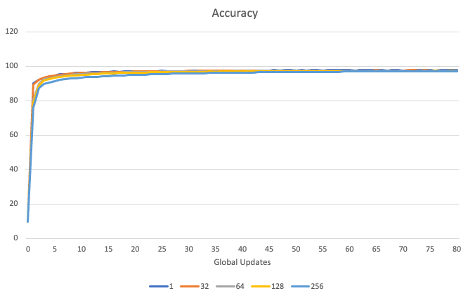
\includegraphics[width=150mm]{thesis/img/res_13.png}
        \caption{Accuracy to estimated convergence for varied $s_{min}$.}
        \label{fig:res_13}
    \end{figure}
    \begin{figure}
        \centering
        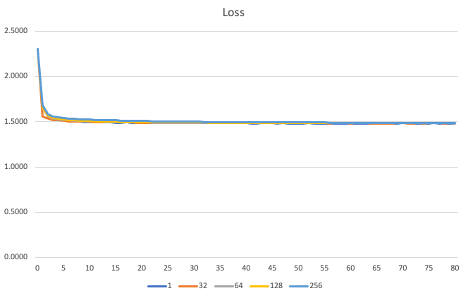
\includegraphics[width=150mm]{thesis/img/res_14.png}
        \caption{Loss to estimated convergence for varied $s_{min}$.}
        \label{fig:res_14}
    \end{figure}
    Zooming in to look at final test accuracy and loss, figures \ref{fig:res_15} \& \ref{fig:res_16} provide slightly more information. Interestingly, our results indicate the median value of 64 batches was most optimal for accuracy, but all the results are once again within .5\% of each other. It does appear, however, that as we approach an even split, or an $s_{min}$ value of 375, final test accuracy takes a slight hit. The results for final update loss are slightly more predictable as the single batch test is the best performer, but again, all values are within 6 thousandths of each other. 
    \begin{figure}
        \centering
        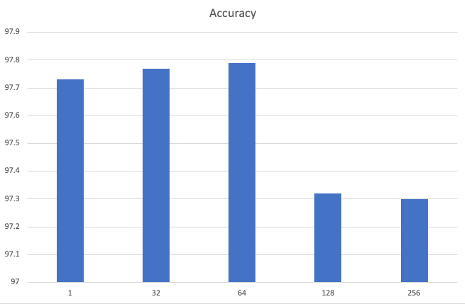
\includegraphics[width=150mm]{thesis/img/res_15.png}
        \caption{80\textsuperscript{th} global update accuracy for varied $s_{min}$.}
        \label{fig:res_15}
    \end{figure}
    \begin{figure}
        \centering
        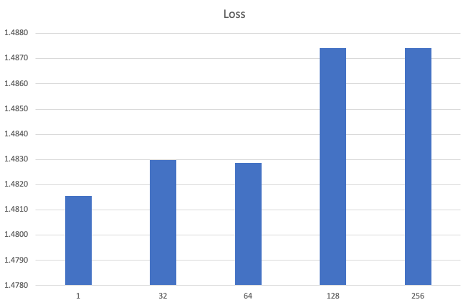
\includegraphics[width=150mm]{thesis/img/res_16.png}
        \caption{80\textsuperscript{th} global update loss for varied $s_{min}$.}
        \label{fig:res_16}
    \end{figure}
    These same experiments were performed during our thesis testing with the exception of $s_{min}$ equal to 256. Since we set beta to its maximum of 8, an equal partition of the dataset capped $s_{min}$ at 234. Similar to our beta testing, figures \ref{fig:res_17} \& \ref{fig:res_18} appear to depict nearly indistinguishable results from the presentation set. 
    \begin{figure}
        \centering
        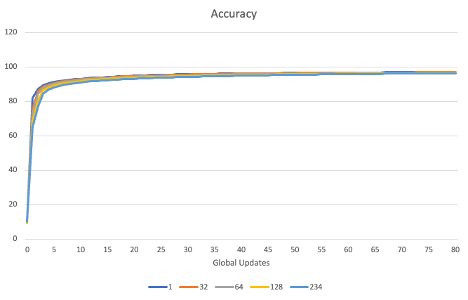
\includegraphics[width=140mm]{thesis/img/res_17.png}
        \caption{Accuracy to estimated convergence for varied $s_{min}$.}
        \label{fig:res_17}
    \end{figure}
    \begin{figure}
        \centering
        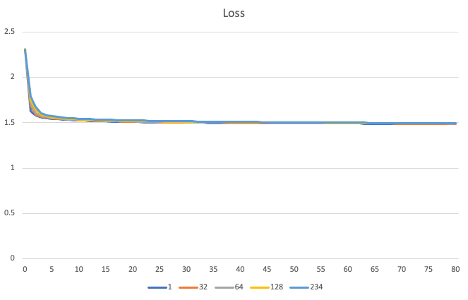
\includegraphics[width=140mm]{thesis/img/res_18.png}
        \caption{Loss to estimated convergence for varied $s_{min}$.}
        \label{fig:res_18}
    \end{figure}
    
    However, when we zoom in to the final test accuracy and loss in figures \ref{fig:res_19} \& \ref{fig:res_20}, we can see our hypothesis may have been more accurate than anticipated. A clear relationship can be drawn between an increasing $s_{min}$ \& decreasing accuracy as well as an increasing $s_{min}$ \& increasing loss. It’s our group’s opinion that the higher beta value of 8 explains these more consistent and expected results. Thankfully, despite the obvious trends, final test accuracy and loss still all fall within <.8\% and 7 thousandths of each other respectively. This affirms the success of FedAvg, and more specifically, our implementation of it.
    
    \begin{figure}
        \centering
        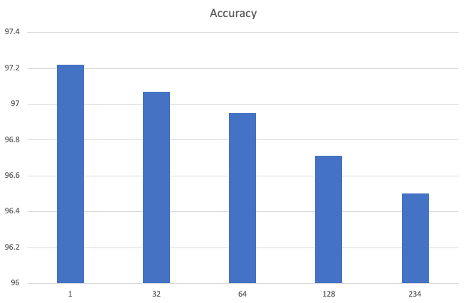
\includegraphics[width=120mm]{thesis/img/res_19.png}
        \caption{80\textsuperscript{th} global update accuracy for varied $s_{min}$.}
        \label{fig:res_19}
    \end{figure}
    \begin{figure}
        \centering
        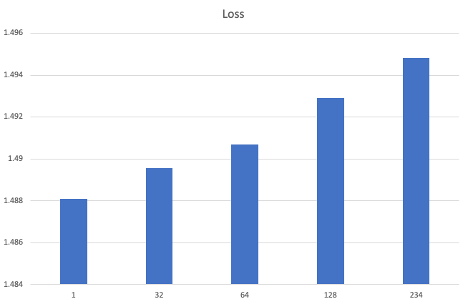
\includegraphics[width=120mm]{thesis/img/res_20.png}
        \caption{80\textsuperscript{th} global update loss for varied $s_{min}$.}
        \label{fig:res_20}
    \end{figure}
\end{document}
